\documentclass[tikz,border=10pt]{standalone}
\usetikzlibrary{shapes.geometric, arrows.meta, positioning}

\tikzset{
    block/.style={rectangle, draw, fill=blue!20, text width=5em, text centered, rounded corners, minimum height=4em},
    input/.style={coordinate},
    output/.style={coordinate},
    arrow/.style={thick,->,>=stealth}
}

\begin{document}
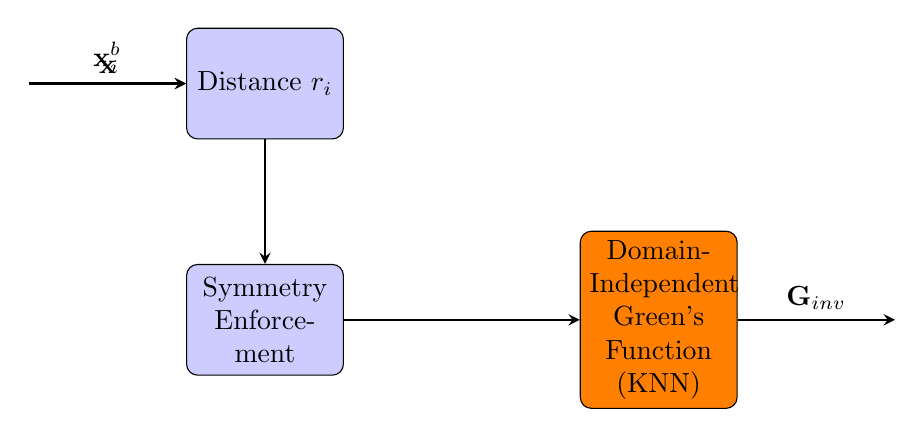
\begin{tikzpicture}[node distance=2cm]

    % Input nodes
    \node[input] (x) {};
    \node[input] at (x.east) (xb) {};

    % Distance node
    \node[block, right of=xb, xshift=1cm] (ri) {Distance $r_i$};

    % Symmetry enforcement node
    \node[block, below of=ri, yshift=-1cm] (symmetry) {Symmetry Enforcement};

    % Domain-invariant Green's function block
    \node[block, right of=symmetry, xshift=3cm, fill=orange] (gknn) {Domain-Independent Green's Function (KNN)};

    % Output node
    \node[output, right of=gknn, xshift=1cm] (y) {};

    % Arrows
    \draw [arrow] (x) -- node[above] {$\mathbf{x}$} (ri);
    \draw [arrow] (xb) -- node[above] {$\mathbf{x}_i^b$} (ri);
    \draw [arrow] (ri) -- (symmetry);
    \draw [arrow] (symmetry) -- (gknn);
    \draw [arrow] (gknn) -- node[above] {$\mathbf{G}_{\text{inv}}$} (y);

\end{tikzpicture}
\end{document}